\documentclass[a4paper]{article}
\usepackage[ngerman]{babel}
\usepackage[utf8]{inputenc}
\usepackage{multicol}
\usepackage{calc}
\usepackage{ifthen}
\usepackage[landscape]{geometry}
\usepackage{amsmath,amsthm,amsfonts,amssymb}
\usepackage{color,graphicx,overpic}
\usepackage{listings}
\usepackage[compact]{titlesec} %less space for headers
\usepackage{mdwlist} %less space for lists
\usepackage[utf8]{inputenc}
\usepackage{tikz}
\usepackage{pdflscape}
\usepackage{verbatim}
\usetikzlibrary{mindmap, arrows,shapes,positioning,shadows,trees}
\tikzstyle{every node}=[draw=black,thin,anchor=west, minimum height=2em]
\usepackage[hidelinks,pdfencoding=auto]{hyperref}
\usepackage{fancyhdr}
\usepackage{lastpage}
\pagestyle{fancy}
\fancyhf{}
\fancyhead[L]{Betriebssysteme}
\fancyfoot[L]{\thepage/\pageref{LastPage}}
\renewcommand{\headrulewidth}{0pt} %obere Trennlinie
\renewcommand{\footrulewidth}{0pt} %untere Trennlinie

\pdfinfo{
    /Title (Betriebssysteme - Cheatsheet)
    /Creator (TeX)
    /Producer (pdfTeX 1.40.0)
    /Author (Robert Jeutter)
    /Subject ()
}

% This sets page margins to .5 inch if using letter paper, and to 1cm
% if using A4 paper. (This probably isn't strictly necessary.)
% If using another size paper, use default 1cm margins.
\ifthenelse{\lengthtest { \paperwidth = 11in}}
    { \geometry{top=.5in,left=.5in,right=.5in,bottom=.5in} }
    {\ifthenelse{ \lengthtest{ \paperwidth = 297mm}}
    {\geometry{top=1.3cm,left=1cm,right=1cm,bottom=1.2cm} }
    {\geometry{top=1.3cm,left=1cm,right=1cm,bottom=1.2cm} }
    }

% Redefine section commands to use less space
\makeatletter
\renewcommand{\section}{\@startsection{section}{1}{0mm}%
                                {-1ex plus -.5ex minus -.2ex}%
                                {0.5ex plus .2ex}%x
                                {\normalfont\large\bfseries}}
\renewcommand{\subsection}{\@startsection{subsection}{2}{0mm}%
                                {-1explus -.5ex minus -.2ex}%
                                {0.5ex plus .2ex}%
                                {\normalfont\normalsize\bfseries}}
\renewcommand{\subsubsection}{\@startsection{subsubsection}{3}{0mm}%
                                {-1ex plus -.5ex minus -.2ex}%
                                {1ex plus .2ex}%
                                {\normalfont\small\bfseries}}
\makeatother

% Don't print section numbers
\setcounter{secnumdepth}{0}

\setlength{\parindent}{0pt}
\setlength{\parskip}{0pt plus 0.5ex}    
% compress space
\setlength\abovedisplayskip{0pt}
\setlength{\parskip}{0pt}
\setlength{\parsep}{0pt}
\setlength{\topskip}{0pt}
\setlength{\topsep}{0pt}
\setlength{\partopsep}{0pt}
\linespread{0.5}
\titlespacing{\section}{0pt}{*0}{*0}
\titlespacing{\subsection}{0pt}{*0}{*0}
\titlespacing{\subsubsection}{0pt}{*0}{*0}

%Tikz global setting
\tikzset{
    topic/.style={
                text centered,
                text width=5cm,
                level distance=1mm,
                sibling distance=5mm,
                rounded corners=2pt
            },
        subtopic/.style={
                yshift=1.5cm,
                text centered,
                text width=3cm,
                rounded corners=2pt,
                fill=gray!10
            },
        theme/.style={
                grow=down,
                xshift=-0.6cm,
                text centered,
                text width=3cm,
                edge from parent path={(\tikzparentnode.205) |- (\tikzchildnode.west)}
            },
        description/.style={
                grow=down,
                xshift=-0.5cm,
                right,
                text centered,
                edge from parent path={(\tikzparentnode.200) |- (\tikzchildnode.west)}
            },
        level 1/.style={sibling distance=5.5cm},
        level 1/.append style={level distance=2.5cm},
}

\begin{document}

\raggedright
\begin{multicols}{3}\scriptsize
  % multicol parameters
  % These lengths are set only within the two main columns
  %\setlength{\columnseprule}{0.25pt}
  \setlength{\premulticols}{1pt}
  \setlength{\postmulticols}{1pt}
  \setlength{\multicolsep}{1pt}
  \setlength{\columnsep}{2pt}

  \centering{
    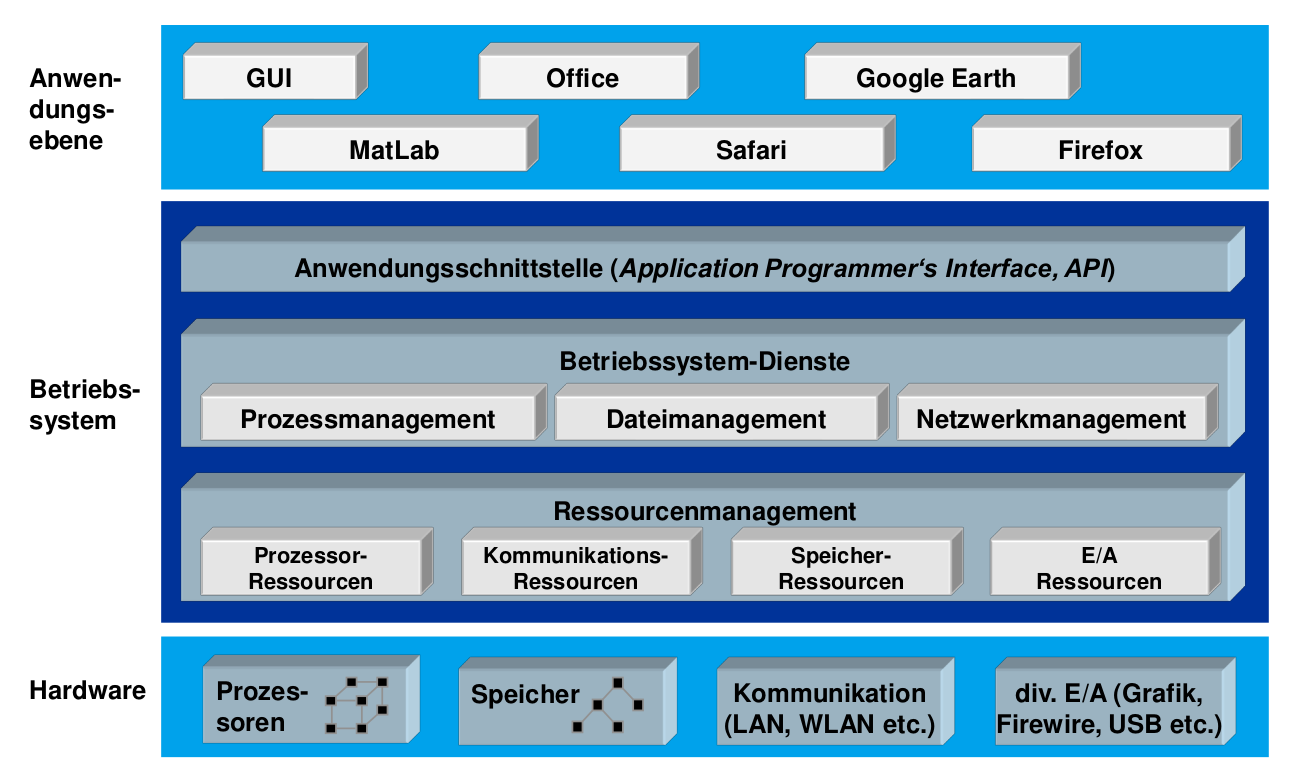
\includegraphics[width=\textwidth/4]{Assets/Betriebssysteme_Uebersicht.png}
  }

  \paragraph{Prozesse}
  \begin{itemize*}
    \item BS-Abstraktionen zur Ausführung von Programmen
    \item Eigentümer von Ressourcen
    \item differenzierte Prozessmodelle: definieren konkrete Prozesseigenschaften
  \end{itemize*}

  \paragraph{Prozessmanagement}
  \begin{itemize*}
    \item Komponente eines Betriebssystems, die Prozessmodell dieses Betriebssystems implementiert
    \item Aufgaben: Prozesserzeugung u. -beendigung (u. Scheduling)
    \item Datenstrukturen: Prozessdeskriptor, -deskriptortabelle
  \end{itemize*}

  \paragraph{Prozessdeskriptor}
  Buchführung über sämtliche zum Management eines Prozesses notwendigen Informationen
  \begin{itemize*}
    \item Prozessidentifikation
    \item Rechtemanagement
    \item Speichermanagement
    \item Prozessormanagement
    \item Kommunikationsmanagement
  \end{itemize*}

  \paragraph{Prozessdeskriptortabelle}
  enthält: Prozessdeskriptoren aller momentan existierenden Prozesse

  \paragraph{Threads}
  BS-Abstraktionen für sequentielle, nebenläufige Aktivitäten; sind Gegenstand des Schedulings

  \paragraph{Multithread-Prozessmodell}
  vollständige Beschreibung einer ablaufenden Aktivität. Dazu gehören insbesondere
  \begin{enumerate*}
    \item das ablaufende Programm
    \item zugeordnete Betriebsmittel (Prozessor/Speicher/Kommunikation)
    \item Rechte
    \item prozessinterne parallele Aktivitäten (Threads) und deren Bearbeitungszustände
  \end{enumerate*}

  \paragraph{Threaddeskriptor}
  ein TCB enthält lediglich:
  \begin{enumerate*}
    \item Threadzustand (aktiv, bereit, blockiert, ...)
    \item Ablaufkontext, falls nicht aktiv (Programmzähler, Stackpointer, Prozessorregister)
  \end{enumerate*}
  enthält nicht: Beschreibung der Ressourcen (Speicherlayout, Rechte)

  \paragraph{Thread-Typen}
  \begin{itemize*}
    \item Kernel Level Threads (KLTs): Kenntnis über Threads: hat Betriebssystem, genauer: der Betriebssystem-Kern(el)
    \item User Level Threads (ULTs): Kenntnis über Threads: existiert nur auf Benutzer-Ebene (user level)
    \item der Betriebssystem-Kern(el) weiß nicht, dass Threads existieren
  \end{itemize*}

  \paragraph{Scheduling}
  Entscheidung: Welche Threads erhalten wann und wie lange einen Prozessor/Prozessorkern zugeteilt?

  \paragraph{Zustandsmodelle}
  Threads können verschiedene Zustände annehmen\\
  Beispiel 3/5-Zustandsmodell)
  \centering{
    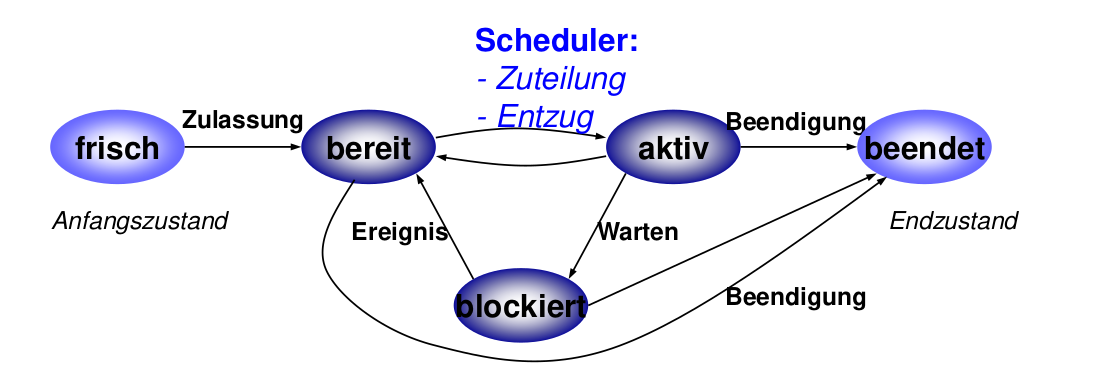
\includegraphics[width=\textwidth/4]{Assets/Betriebssysteme_Zustandsmodell.png}
  }

  \paragraph{Scheduling: Notwendigkeit u. Sinn}
  \begin{itemize*}
    \item allg: Anzahl Aktivitäten $>>$ Anzahl Prozessoren
    \item nicht alle können gleichzeitig arbeiten
    \item eine Auswahl muss getroffen werden
    \item Auswahlstrategie: Schedulingstrategie, -Algorithmus
  \end{itemize*}

  \paragraph{Scheduling-Strategien}
  \begin{itemize*}
    \item abhängig vom Einsatzfeld eines Betriebssystems
    \begin{itemize*}
      \item Echtzeitsysteme: Einhaltung von Fristen
      \item interaktive Systeme: Reaktivität
    \end{itemize*}
    \item wichtige Strategien:
    \begin{itemize*}
      \item FCFS (First Come, First Served)
      \item SRTN (Shortest Remaining Time Next)
      \item Round Robin (ohne und mit Prioritäten)
      \item EDF (earliest deadline first)
      \item ratenmonotones Scheduling
    \end{itemize*}
  \end{itemize*}

  \paragraph{Privilegierungsebenen}
  \begin{itemize*}
    \item sind typischerweise 'kernel mode' und 'user mode'
    \item steuern Rechte
    \begin{itemize*}
      \item zur Ausführung privilegierter Prozessorinstruktionen
      \item zur Konfiguration des Arbeitsspeicherlayouts
      \item zum Zugriff auf Arbeitsspeicherbereiche
      \item zum Zugriff auf E/A-Geräte
    \end{itemize*}
    \item Durchsetzung von Regeln: "Nur ein im 'kernel mode' ablaufender Prozess hat Zugriff auf ..."
  \end{itemize*}

  \paragraph{Kommunikation und Synchronisation}
  \begin{itemize*}
    \item Austausch von Daten zwischen Prozessen = Kommunikation (Inter-Prozess-Kommunikation, IPC)
    \item Abweichende Geschwindigkeiten von Sender und Empfänger: behandelt durch Synchronisation
  \end{itemize*}

  \paragraph{kritischer Abschnitt}
  \begin{itemize*}
    \item in kritischen Abschnitt darf stets nur ein Thread sein
    \item notwendig: wechselseitiger (gegenseitiger) Ausschluss
    \item realisiert durch Entry- und Exit-Code z.B. die Semaphor-Operationen belegen (P) und freigeben (V)
  \end{itemize*}

  \paragraph{Mechanismen zur Synchronisation}
  \begin{itemize*}
    \item binäre Semaphore und mehrwertige Semaphore
    \item (Hoar‘sche) Monitore
  \end{itemize*}

  \paragraph{Mechanismen zur Kommunikation}
  \begin{itemize*}
    \item Shared Memory (gemeinsamer Speicher)
    \item Botschaften
    \item Fernaufrufe
    \item Systemaufrufe
  \end{itemize*}

  \paragraph{Notwendigkeit des Ereignismanagement}
  \begin{itemize*}
    \item in BS laufen sehr viele Aktivitäten parallel ab
    \item dabei entstehen immer wieder Situationen, in denen auf unterschiedlichste Ereignisse reagiert werden muss, z.B.
    \begin{itemize*}
      \item Timerablauf
      \item Benutzereingaben (Maus, Tastatur)
      \item Eintreffen von Daten von Netzwerken, Festplatten, ...
      \item Einlegen/-stecken von Datenträgern
      \item Aufruf von Systemdiensten
      \item Fehlersituationen
    \end{itemize*}
  \end{itemize*}

  \paragraph{Umgangsformen mit Ereignissen}
  \begin{itemize*}
    \item 'busy waiting'
    \item 'periodic testing'
    \item Unterbrechungen ('Interrupts')
  \end{itemize*}

  \paragraph{Programmiermodelle für Interrupts}
  \begin{itemize*}
    \item Prozeduren ($\rightarrow$ inline Prozeduraufrufmodell)
    \item IPC-Operationen ($\rightarrow$ IPC-Modell)
    \item Threads ($\rightarrow$ pop-up Thread Modell)
  \end{itemize*}

  \paragraph{Interrupts auf Anwendungsebene}
  \begin{itemize*}
    \item notwendig: Event Service Routines (ESRs)
    \item Beispiel: UNIX/Linux-Signalbehandlung
  \end{itemize*}

  \paragraph{Virtuelle Prozessadressräume und physischer Adressraum, Abbildungen}
  \centering{
    \includegraphics[width=\textwidth/4]{Assets/Betriebssysteme_Adressräume.png}
  }

  \paragraph{Seitenabbildungstabellen}
  \centering{
    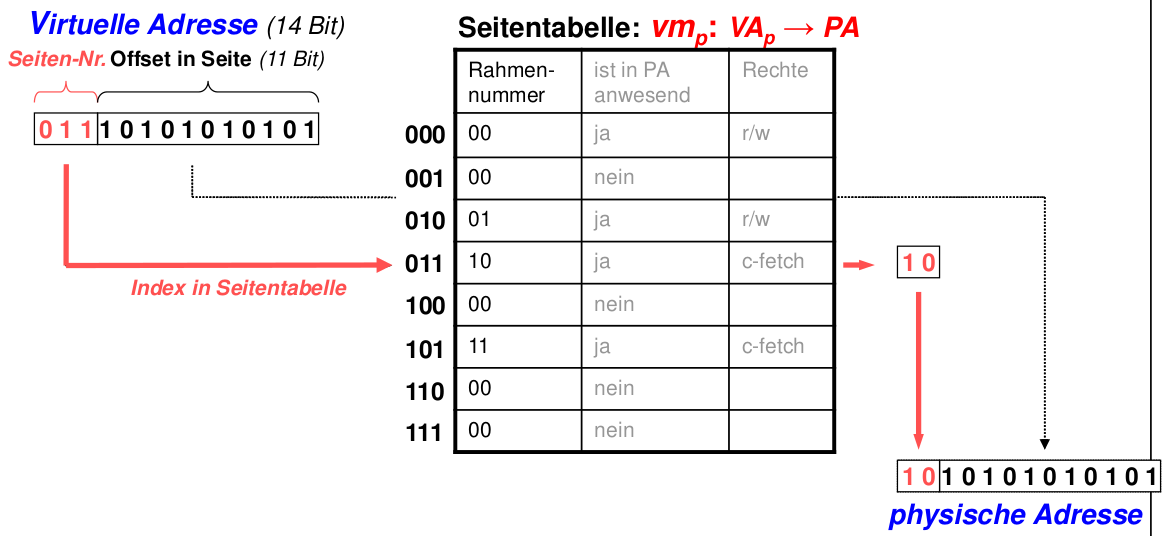
\includegraphics[width=\textwidth/4]{Assets/Betriebssysteme_Seitenabbildungstabellen.png}
  }

  \paragraph{Seitentabelleneinträge}
  \centering{
    \includegraphics[width=\textwidth/4]{Assets/Betriebssysteme_Seitentabelleneinträge.png}
  }
  \begin{itemize*}
    \item anwesend: liegt Seite im Arbeitsspeicher? ('present'-Bit)
    \item benutzt: wurde auf die Seite zugegriffen? ('used'-Bit)
    \item verändert: ist Seite 'schmutzig'? ('dirty/modified'-Bit)
    \item Schutz: erlaubte Zugriffsart je Privilegierungsebene ('access control list')
    \item Caching: darf Inhalt der Seite gecached werden?
  \end{itemize*}

  \paragraph{Seitenaustauschalgorithmen}
  \begin{itemize*}
    \item Optimal: Auslagern der Arbeitsspeicherseite, deren
    \begin{itemize*}
      \item nächster Gebrauch am weitesten in der Zukunft liegt
      \item Auslagerung nichts kostet
    \end{itemize*}
    \item einige Algorithmen, die sich diesem Optimum annähern:
    \begin{itemize*}
      \item First-In, First-Out (FIFO)
      \item Second-Chance
      \item Least Recently Used (LRU)
      \item Working Set / WSClock
    \end{itemize*}
  \end{itemize*}

  \paragraph{i-Node}
  Metainformationen über genau eine Datei
  \centering{
    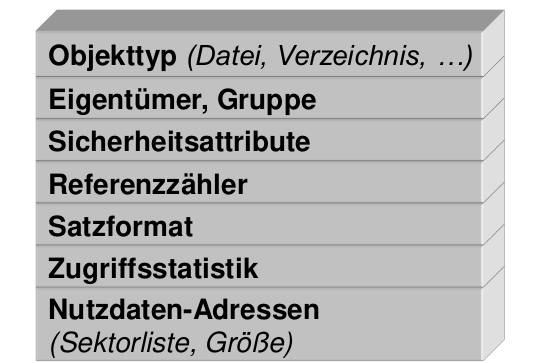
\includegraphics[width=\textwidth/6]{Assets/Betriebssysteme_i-Node.png}
  }

  \paragraph{Verzeichnis}
  = Menge von Paaren (Name, i-Node-Index)

  \paragraph{Superblock} = Einstiegspunkt eines Dateisystems. Enthält Schlüsselparameter:
  \begin{itemize*}
    \item Name des Dateisystems
    \item Typ (NTFS, Ext * , HFS, ...) → Layout der Metadaten
    \item Größe und Anzahl Sektoren
    \item Ort und Größe der i-Node-Tabelle
    \item Ort und Größe der Freiliste
    \item i-Node-Nummer des Wurzelverzeichnisses
  \end{itemize*}

  \paragraph{Hardware-Prinzipien}
  \begin{itemize*}
    \item Controller-Register
    \begin{itemize*}
      \item in E/A-Adressräumen
      \item im Arbeitsspeicher (Memory Mapped E/A)
      \item Isolation, Robustheit, Sicherheit
    \end{itemize*}
    \item Interruptsystem: asynchrone Benachrichtigungen
  \end{itemize*}

  \paragraph{Software-Prinzipien}
  Gerätemanager (Treiber)
  \begin{itemize*}
    \item Auftragsmanagement
    \item ISRs
  \end{itemize*}

  \paragraph{Betriebssystem-Architekturen}
  \centering{
    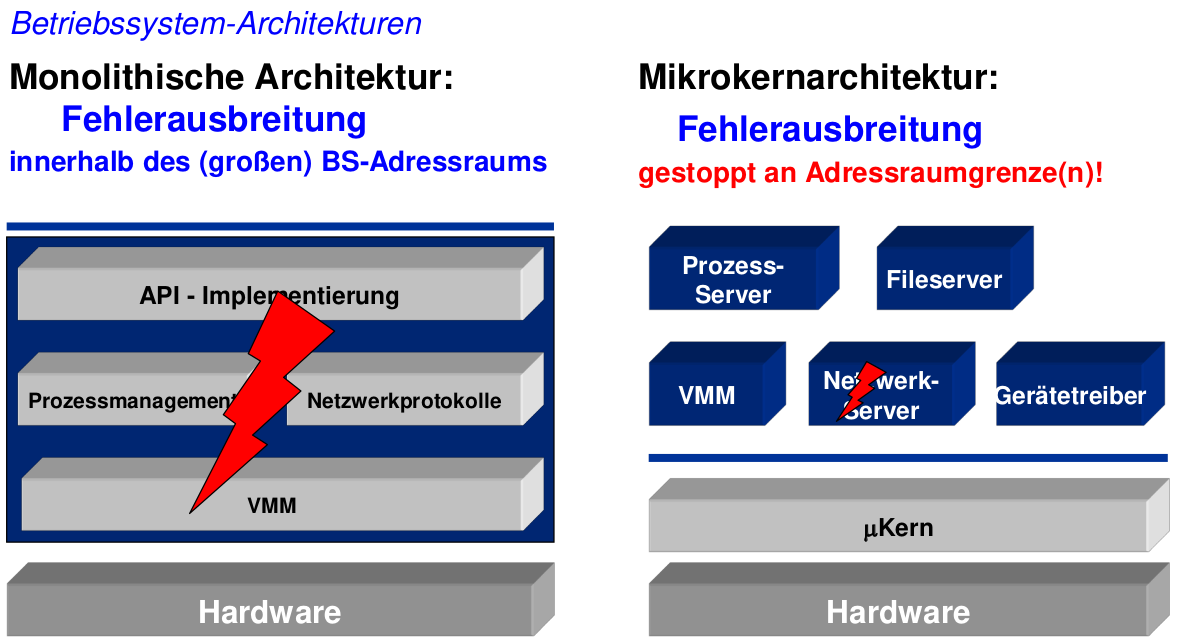
\includegraphics[width=\textwidth/4]{Assets/Betriebssysteme_Architekturen.png}
  }

  \paragraph{SELinux-Ansatz} neue Betriebssystem-Abstraktion
  \begin{itemize*}
    \item absolute Kontrolle über kritische Funktionen des Betriebssystems
    \item spezifiziert durch Regelmenge
    \item implementiert durch die SELinux-Sicherheitsarchitektur
  \end{itemize*}

  \paragraph{Robustheit} Tolerierung unvorhergesehener Fehler und Ausfälle
  \begin{itemize*}
    \item Mikrokernarchitekturen (Robuster als Makrokern)
    \item Fehlerisolation
    \item Möglichkeiten zur Fehlerbehebung (z.B. Micro-Reboot)
  \end{itemize*}

  \paragraph{Funktionale Eigenschaften}
  \begin{itemize*}
    \item Authentisierung, Verschlüsselung
    \item Informations-management
    \item Kommunikations-management
    \item Ressourcen-management
  \end{itemize*}

  \paragraph{Nichtfunktionale Eigenschaften}
  \begin{itemize*}
    \item     Sicherheit
    \item Korrektheit
    \item Echtzeitfähigkeit
    \item Skalierbarkeit
    \item Offenheit
    \item Sparsamkeit
    \item Verfügbarkeit
    \item Robustheit
  \end{itemize*}

  \paragraph{Betriebssysteme}
  \begin{itemize*}
    \item     Mainframe
    \begin{itemize*}
      \item performante E/A
      \item Massen-daten-verarbeitung
    \end{itemize*}
    \item Server (Web Server, Fileshare)
    \item Parallelrechner
    \begin{itemize*}
      \item parallele Algorithmen, hoher Rechenbedarf
      \item schnelle IPC
    \end{itemize*}
    \item Desktop/Laptop
    \item Echtzeit
    \item Eingebettete
  \end{itemize*}


\end{multicols}


%%%%%%%%%%%%%%%%%%%%%%%%%%%%%%%%%%%%%%%% Überblick
\begin{tikzpicture}[
    topic/.style={
        minimum height=8mm,
        text depth = 0pt,
        text centered,
        text width=5cm,
        level distance=1mm,
        sibling distance=5mm,
        rounded corners=2pt},
    subtopic/.style={
        yshift=1.5cm,
        text centered,
        text width=3cm,
        rounded corners=2pt,
        fill=gray!10},
    theme/.style={
        grow=down,
        xshift=-0.6cm,
        text centered,
        text width=3cm,
        edge from parent path={(\tikzparentnode.205) |- (\tikzchildnode.west)}},
    level1/.style ={level distance=1cm},
    level2/.style ={level distance=2cm},
    level3/.style ={level distance=3cm},
    level4/.style ={level distance=4cm},
    level5/.style ={level distance=5cm},
    level6/.style ={level distance=6cm},
    level 1/.style={sibling distance=4cm},
    level 1/.append style={level distance=3cm},
  ]
  % Topic
  \node[topic]{Betriebssysteme}
  % Subtopic and Themes
  child{ node [subtopic] {Prozessor-management}
      child[theme,level distance=1cm]{ node {Prozesserzeugung}}
      child[theme,level distance=2cm]{ node {Prozess-terminierung}}
      child[theme,level distance=3cm]{ node {Threads}}
    }
  child{ node [subtopic] {Scheduling}
      child[theme,level distance=1cm]{ node {Scheduler-aktivierung}}
      child[theme,level distance=2cm]{ node {Scheduling Strategien}}
    }
  child{ node [subtopic] {Privilegierungs-ebenen}}
  child{ node [subtopic] {Kommunikation \& Synchronisation}
      child[theme,level distance=1cm]{ node {Elementare Konzepte}}
      child[theme,level distance=2cm]{ node {wechselseitiger Ausschluss}}
      child[theme,level distance=3cm]{ node {Mechanismen}}
    }
  child{ node [subtopic] {Speicher-management}
      child[theme,level distance=1cm]{ node {Speicher-technologien}}
      child[theme,level distance=2cm]{ node {Speicher-klassen}}
      child[theme,level distance=3cm]{ node {Relokation}}
      child[theme,level distance=4cm]{ node {Swapping}}
      child[theme,level distance=5cm]{ node {Virtueller Speicher}}
      child[theme,level distance=6cm]{ node {Segmentierung}}
    }
  child{ node [subtopic] {Dateisystem}
      child[theme,level distance=1cm]{ node {Dateimodelle}}
      child[theme,level distance=2cm]{ node {Dateisysteme}}
      child[theme,level distance=3cm]{ node {Datenstrukturen \& Algorithmen}}
    };
\end{tikzpicture}


%%%%%%%%%%%%%%%%%%%%%%%%%%%%%%%%%%%%%% Prozessormanagement
\begin{tikzpicture}[
    level 1/.style={sibling distance=5.5cm},
    level 1/.append style={level distance=2.5cm},
  ]
  % Topic
  \node[topic]{Prozessormanagement}
  % Subtopic and Themes
  child{ node [subtopic] {Aufgaben}
      child[theme,level distance=1cm]{node{Prozess-identifikation}}
      child[theme,level distance=2cm]{node{Scheduling}}
      child[theme,level distance=3cm]{node{Ereignis-management}}
      child[theme,level distance=4cm]{node{Rechte-management}}
      child[theme,level distance=5cm]{node{Speicher-management}}
      child[theme,level distance=6cm]{node{Prozessor-management}}
      child[theme,level distance=7cm]{node{Kommunikations-management}}
      child[theme,level distance=8cm]{node{Virtueller Adressraum}}
      child[theme,level distance=9cm]{node{allg Ressourcen Management}}
    }
  child{ node [subtopic] {Prozesserzeugung}
      child[theme,level distance=1cm]{ node {Vorraussetzungen}
          child[description,level distance=1cm]{ node {Rechte}}
          child[description,level distance=2cm]{ node {Ressourcen Verfügbar}}
          child[description,level distance=3cm]{ node {Sicherheit}}
          child[description,level distance=4cm]{ node{Fariness}}
          child[description,level distance=5cm]{node{Robustheit / Überlastvermeidung}}
        }
      child [theme,level distance=7cm]{ node {Namens-vergabe}
          child[description,level distance=1cm]{node{eindeutig bzgl allen existierenden}}
          child[description,level distance=2cm]{node{nicht eindeutig bzgl allen}}
        }
      child [theme,level distance=10cm]{ node {Stammbaumpflege}
          child[description,level distance=1cm]{node{erzeugt Kinder}}
          child[description,level distance=2cm]{node{baumartige Hierarchie}}
          child[description,level distance=3cm]{node{Verwaiste Prozesse $->$ Adoption}}
        }
      child [theme,level distance=14cm]{ node {Allokation (von Ressourcen)}
          child[description,level distance=1cm]{node{Arbeits-speicher Größe}}
          child[description,level distance=2cm]{node{Zeitpunkt}}
          child[description,level distance=3cm]{node{Prozessorzeit}}
          child[description,level distance=4cm]{node{Format}}
        }
    }
  child{ node [subtopic] {Prozessterminierung}
      child[theme,level distance=1cm]{node{durch}
          child[description,level distance=1cm]{node{Aufgabe erledigt}}
          child[description,level distance=2cm]{node{Fehler aufgetreten}}
          child[description,level distance=3cm]{node{durch Nutzer geschlossen}}
        }
      child[theme,level distance=5cm]{node{Folgen}
          child[description,level distance=1cm]{node{Freigabe der Ressourcen}}
          child[description,level distance=2cm]{node{Benachrichtigung der 'Parents'}}
          child[description,level distance=3cm]{node{Adoption der 'Children'}}
        }
    }
  child{ node [subtopic] {Threads}
      child[theme,level distance=1cm]{node{sequenziell innerhalb eines Prozesses}}
      child[theme,level distance=3cm]{node{Kernel Level Thread}
          child[description,level distance=1cm]{node{Implementiert im Betriebssystem}}
          child[description,level distance=2cm]{node{Betriebssystem hat Kenntnis über Thread}}
          child[description,level distance=3cm]{node{Multi-Thread-modell}}
          child[description,level distance=4cm]{node{Performance durch Parallelität}}
          child[description,level distance=5cm]{node{Nutzung von Mehrkern-architektur}}
        }
      child[theme,level distance=10cm]{node{User Level Thread}
          child[description,level distance=1cm]{node{Implementiert auf Anwendungsebene}}
          child[description,level distance=2cm]{node{Kenntnis nur bei Endbenutzer}}
          child[description,level distance=3cm]{node{Single-Thread-Modell}}
          child[description,level distance=4cm]{node{Performance durch geringen Overhead}}
          child[description,level distance=5cm]{node{management ohne systemaufrufe}}
          child[description,level distance=6cm]{node{Individualität}}
          child[description,level distance=7cm]{node{Portabilität}}
        }
    };
\end{tikzpicture}


%%%%%%%%%%%%%%%%%%%%%%%%%%%%%%%%%%%%%%%% Scheduling
\begin{tikzpicture}[
    level 1/.style={sibling distance=4.6cm},
    level 1/.append style={level distance=3cm},
  ]
  % Topic
  \node[topic]{Scheduling}
  % Subtopic and Themes
  child{ node [subtopic] {Aktivierung}
      child[theme,level distance=1cm]{node{Threadzustände im 3/5 Modell}
          child[description,level distance=1cm]{node{bereit: kann aktiv werden}}
          child[description,level distance=2cm]{node{aktiv: arbeitet}}
          child[description,level distance=3cm]{node{blockiert: wartet auf Ereignis}}
          child[description,level distance=4cm]{node{frisch: erzeugt, Rechte fehlen}}
          child[description,level distance=5cm]{node{beendet: in Freigabephase}}
        }
      child[theme,level distance=7cm]{node{Entscheidung Überprüfen bei}
          child[description,level distance=1.5cm]{node{Prozess/Thread Erzeugung/Terminierung}}
          child[description,level distance=3cm]{node{Ereignis eintritt}}
          child[description,level distance=4cm]{node{Wechsel von Prioritäten}}
          child[description,level distance=5cm]{node{periodisch}}
        }
    }
  child{node[subtopic]{Ziele}
      child[theme,level distance=1cm]{node{abhängig von Einsatz des Betriebssystems}}
      child[theme,level distance=2.5cm]{node{ergänzt durch allg Ziele}}
      child[theme,level distance=3.5cm]{node{Einhaltung von Fristen}}
      child[theme,level distance=5cm]{node{Minimieren der Thread/Prozess-wechsel}}
    }
  child { node [subtopic]{Batch-System}
      child[theme,level distance=1cm]{node{Auslastung teurer Betriebsmittel (CPU)}}
      child[theme,level distance=3cm]{node{Minimierung der Scheduling Kosten (wenig Wechsel, kurze Laufzeiten)}}
      child[theme,level distance=5cm]{node{Maximierung des Durchsatzes (erledigte Arbeit/Zeit)}}
      child[theme,level distance=6.5cm]{node{First Come First Served}
          child[description,level distance=1cm]{node{in Reihenfolge der rechenbereiten}}
          child[description,level distance=2cm]{node{sehr einfach, guter durchsatz}}
          child[description,level distance=3cm]{node{nicht immer klug}}
        }
      child[theme,level distance=10cm]{node{Shortest Remaining Time Next}
          child[description,level distance=1cm]{node{Thread mit vorr. kürzester Restrechenzeit}}
          child[description,level distance=2.5cm]{node{preemtiv; konkurrrierende Threads verdrängen}}
          child[description,level distance=4cm]{node{Restlaufzeit muss vorliegen}}
        }
    }
  child { node [subtopic]{Interaktives System}
      child[theme,level distance=1cm]{node{Benutzer kann eingreifen}}
      child[theme,level distance=2cm]{node{Minimierung von Reaktionszeiten}}
      child[theme,level distance=3cm]{node{Fairness (mehrere Benutzer)}}
      child[theme,level distance=4cm]{node{Round Robin Varianten}
          child[description,level distance=1cm]{node{jeder Thread gleicher Teil der Zeitscheibe}}
          child[description,level distance=2.5cm]{node{einfach zu implementieren}}
          child[description,level distance=3.5cm]{node{geringe Algorithmuskosten}}
          child[description,level distance=4.5cm]{node{schnelle Entscheidungen}}
          child[description,level distance=5.5cm]{node{geringes Wissen notwendig}}
        }
    }
  child{node[subtopic]{Prioritäten}
      child[theme,level distance=1cm]{node{jeder Thread erhält indv. Priorität}}
      child[theme,level distance=2.5cm]{node{höchste Prioritäten erhalten Prozessor}}
      child[theme,level distance=4cm]{node{gleiche Priorität: Round Robin}}
    }
  child{node[subtopic]{in Echtzeitsystemen}
      child[theme,level distance=1cm]{node{EDF: earliest deadline first}
          child[description,level distance=1cm]{node{dynamische Lasten; adaptiv}}
          child[description,level distance=2cm]{node{Threads nennen Deadline/Frist}}
          child[description,level distance=3cm]{node{kausale und zeitliche Unabhängigkeit}}
          child[description,level distance=4cm]{node{Priorität setzt kürzere Fristen}}
        }
      child[theme,level distance=7cm]{node{RMS: rate-monotonic scheduling}
          child[description,level distance=1cm]{node{periodische Lasten}}
          child[description,level distance=2cm]{node{Threads nennen Periodendauer}}
          child[description,level distance=3cm]{node{kürzeste Periodendauer aktiv}}
          child[description,level distance=4cm]{node{statische Prioritäten}}
        }
    };
\end{tikzpicture}

%%%%%%%%%%%%%%%%%%%%%%%%%%%%%%%%%%%%%%%% Privilegierungsebenen
\begin{tikzpicture}[
    level 1/.style={sibling distance=5cm},
    level 1/.append style={level distance=3cm},
  ]
  % Topic
  \node[topic]{Privilegierungsebenen}
  % Subtopic and Themes    
  child{node[subtopic]{Konzepte}
      child[theme,level distance=1cm]{node{private Adressräume}}
      child[theme,level distance=3cm]{node{Zugriffsschutz auf Arbeitsspeicherbereiche}}
    }
  child{node[subtopic]{kritische Operationen}
      child[theme,level distance=1cm]{node{Abschalten der Uhr}}
      child[theme,level distance=2cm]{node{Abschalten des Ereignismanagement}}
      child[theme,level distance=3cm]{node{Veränderung des Speicherlayouts}}
      child[theme,level distance=4.3cm]{node{Veränderng kritischer Prozessorkontrollregister}}
      child[theme,level distance=5.5cm]{node{Zugriff auf E/A Geräte}}
    }
  child{node[subtopic]{P. Ebenen}
      child[theme,level distance=1cm]{node{steuern Rechte}
          child[description,level distance=1cm]{node{zur Ausführung privilegierter Prozessorinstruktionen}}
          child[description,level distance=2.5cm]{node{zur Konfiguration des Arbeitsspeicher-Layouts}}
          child[description,level distance=3.8cm]{node{zum Zugriff auf Arbeitsspeicherbereiche}}
          child[description,level distance=5cm]{node{zum Zugriff auf E/A-Geräte}}
        }
      child[theme,level distance=7cm]{node{realisiert in Ringen (0-3)}}
    }
  child{node[subtopic]{Implementierung}
      child[theme,level distance=1cm]{node{Hardware Unterstützung}}
      child[theme,level distance=3cm]{node{Teil "Current Privilege Level" (CPL)}}
      child[theme,level distance=5cm]{node{permantente Überwachung}}
      child[theme,level distance=7cm]{node{Änderung der CPL beschränken}}
    }
  child{node[subtopic]{Botschaften}
      child[theme,level distance=1.3cm]{node{P.E. $< 3$ ablaufende Aktivität hat Zugriff auf kritische Ressourcen}}
      child[theme,level distance=3cm]{node{P.E. 0 ablaufende Aktivität hat Zugriff auf}
          child[description,level distance=1cm]{node{Ressourcen eines Prozessors}}
          child[description,level distance=2.5cm]{node{MMU-Register zur Arbeitsspeicherkonfiguration}}
          child[description,level distance=4cm]{node{Register der E/A-Peripherie}}
        }
    };
\end{tikzpicture}


%%%%%%%%%%%%%%%%%%%%%%%%%%%%%%%%%%%%%%%% Kommunikation und Synchronisation
\begin{tikzpicture}[
    level 1/.style={sibling distance=5cm},
    level 1/.append style={level distance=3cm},
  ]
  % Topic
  \node[topic]{Kommunikation und Synchronisation}
  % Subtopic and Themes          
  child { node [subtopic]{Elementare Konzepte}
      child[theme,level distance=1.5cm]{node{nur 1 Thread pro Speicherbereich arbeiten}}
      child[theme,level distance=3cm]{node{Austausch von Daten zwischen Prozessen $\rightarrow$ Kommunikation}}
      child[theme,level distance=5cm]{node{Abweichende Geschwindigkeiten von Sender und Empfänger $\rightarrow$ Synchronisation}}
      child[theme,level distance=7.5cm]{node{Eine Phase, in der ein Thread eine exklusive Operation auf einer Ressource ausführt, heißt kritischer Abschnitt.}}
      child[theme,level distance=10cm]{node{Kritische Abschnitte erfordern den wechselseitigen Ausschluss (die Isolation) konkurrierender Threads bzw. Prozesse.}}
    }
  child { node [subtopic]{wechselseitiger Ausschluss}
      child[theme,level distance=1.5cm]{node{Korrektheit: in kritischen Abschnitt höchstens ein Thread}}
      child[theme,level distance=4cm]{node{Lebendigkeit: Falls ein Thread einen kritischen Abschnitt betreten möchte, dann betritt (irgendwann) ein Thread diesen Abschnitt.}}
      child[theme,level distance=7.5cm]{node{Verhungerungs-freiheit: Kein Thread wartet für immer vor einem kritischen Abschnitt}}
    }
  child { node[subtopic] {(binäre) Semaphore}
      child[theme,level distance=1cm]{node{2 Zustände: frei, belegt}}
      child[theme,level distance=2cm]{node{2 atomare Operationen P/V}}
      child[theme,level distance=3.5cm]{node{Sämtliche Nutzer dieses kritischen Abschnitts müssen diese semaphore verwenden}}
      child[theme,level distance=5cm]{node{Unterstützung durch Hardware: die TSL-Operation (TestAndSetLock)}}
      child[theme,level distance=6.5cm]{node{Implementierung im Ressourcenmanagement}}
      child[theme,level distance=9cm]{node{Mehrwertiger Semaphor: bestimmt maximale Anzahl von Threads, die gleichzeitig aktiv sein können}}
    }
  child { node [subtopic]{Hoare'sche Monitore}
      child[theme,level distance=1.5cm]{node{Zusammenfassen von Daten/Operationen/Zugriff zu abstrakten Datentyp}}
      child[theme,level distance=3.5cm]{node{Zugriff auf Daten über implizit synchronisierende Operation}}
      child[theme,level distance=5.3cm]{node{kritischer Abschnitt und Daten in durch Monitor geschütztem Bereich}}
      child[theme,level distance=6.8cm]{node{wechselseitiger Ausschluss}}
      child[theme,level distance=8cm]{node{je Monitor eine Semaphor}}
      child[theme,level distance=9cm]{node{am Eingang eine P-Operation}}
      child[theme,level distance=10cm]{node{am Ausgang eine V-Operation}}
    }
  child { node[subtopic] {weitere Mechanismen}
      child [theme,level distance=1cm]{ node {Trans-aktionaler Speicher}
          child[description,level distance=1cm]{node{keine Sperre bei Ausschluss $\rightarrow$ Parallelität}}
          child[description,level distance=2.5cm]{node{nach Operation untersuchen auf Fehler und Korrektur}}
          child[description,level distance=4cm]{node{Kombination mit Transaktionen}}
        }
      child [theme,level distance=6cm]{ node {Botschaften}
          child[description,level distance=1cm]{node{Komm. zw. Prozessen innerhalb eines Systems}}
          child[description,level distance=2cm]{node{Senden/Empfangen von Botschaften}}
          child[description,level distance=3cm]{node{Kommunikationsparadigma}}
        }
      child [theme,level distance=10cm]{ node {Fernaufrufe (Remote Procedure Calls)}}
      child [theme,level distance=11cm]{ node {System-aufrufe}}
      child [theme,level distance=12cm]{ node {Ereignis-management}}
      child [theme,level distance=13cm]{ node {IPC Modell}}
      child [theme,level distance=14cm]{ node {pop-up-Thread-Modell}}
    };
\end{tikzpicture}

%%%%%%%%%%%%%%%%%%%%%%%%%%%%%%%%%%%%%%%% Speichermanagement
\begin{tikzpicture}[
  level 1/.style={sibling distance=5cm},
  level 1/.append style={level distance=3cm},
]
% Topic
\node[topic]{Virtueller Speicher}
% Subtopic and Themes          
child { node [subtopic]{Virtuelles Speichermanagement}}
child { node [subtopic]{Abbildung}}
child { node [subtopic]{Memory Management Units}}
child { node [subtopic]{Seiten-abbildungs-tabellen}}
child { node [subtopic]{Seiten-austausch-Algorithmen}
    child [theme,level distance=1cm]{ node {FIFO}}
    child [theme,level distance=2cm]{ node {Second Chance}}
    child [theme,level distance=3cm]{ node {Least Recently Used}}
    child [theme,level distance=4cm]{ node {Working Set}}
    child [theme,level distance=5cm]{ node {WSClock}}
  };
\end{tikzpicture}

\end{document}